\documentclass{bredelebeamer}

%%%%%%%%%%%%%%%%%%%%%%%%%%%%%%%%%%%%%%%%%%%%%%%%

\title[Programación en MatLAB]{Introducción a la programación con MatLAB}
\subtitle{Módulo 01 - Ámbiente de Matlab}

\author{- AUTORES - \inst{1}}
\institute[UNIVERSIDAD]
{
  \inst{1}%
  - NOMBRE UNIVERSIDAD - 
  }

\date{AÑO}

\subject{Taller de programación}

\logo{

\includegraphics[scale=0.15]{images/logo.png}
}

%%%%%%%%%%%%%%%%%%%%%%%%%%%%%%%%%%%%%%%%%%%%%%%%%%%%%%%%%%%%%%%%%%%%%
\begin{document}

\begin{frame}
  \titlepage 
\end{frame}

%%%%%%%%%%%%%%%%%%%%%%%%%%%%%%%%%%%%%%%%%%%%%%%%%%%%%%%%%%%%%%%%%%%%%

% Sección de ambiente MATLAB

%%%%%%%%%%%%%%%%%%%%%%%%%%%%%%%%%%%%%%%%%%%%%%%%%%%%%%%%%%%%%%%%%%%%%

\section{Ambiente Matlab}

\begin{frame}{Entorno de trabajo}
\begin{center}
Pantalla de entrada de Matlab
\end{center}
\begin{center}
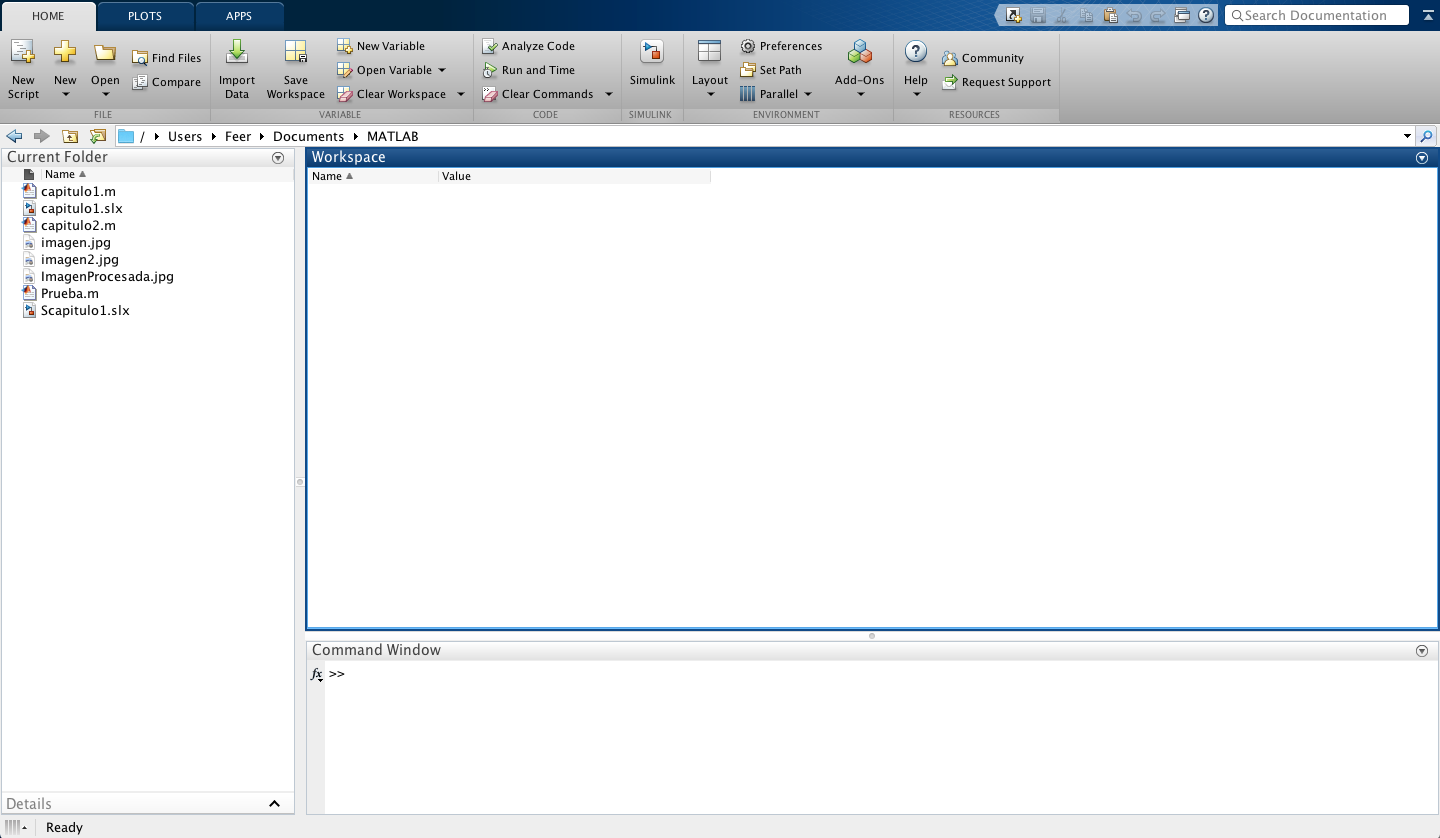
\includegraphics[scale=0.17]{images/pantalla1.png}
\end{center}
\end{frame}

\begin{frame}{Entorno de trabajo}
Los elementos más importantes de esta pantalla son:\\
\begin{itemize}
\item Command Window (ventana de comandos)
\item Command History (historial de comandos)
\item Current Directory (directorio actual)
\item Workspace (espacio de trabajo)
\item Help (ayuda)
\end{itemize}
\end{frame}

\begin{frame}{Command window}
Command window: Ejecuta las funciones MATLAB\\
\begin{center}
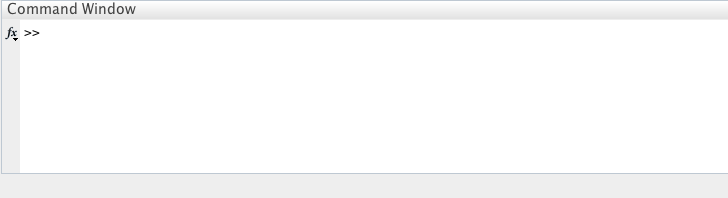
\includegraphics[scale=0.3]{images/pantalla2.png}
\end{center}
Ej. Ejecutar las siguiente líneas. Obtener conclusiones.
\lstinputlisting[xleftmargin=.4\textwidth]{scripts/ej1.m}
\begin{exampleblock}{Comando}
Ver comando: \textbf{clc}
\end{exampleblock}
\end{frame}

\begin{frame}{Command history}
Registra los comandos que se escriben en la ventana de comandos.
\begin{center}
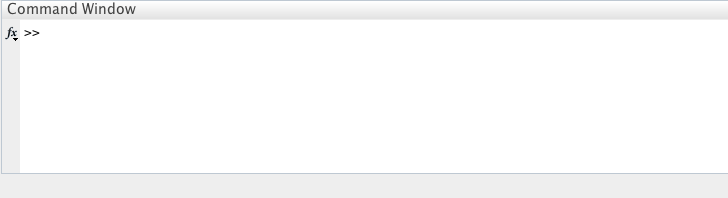
\includegraphics[scale=0.3]{images/pantalla2.png}
\end{center}
\end{frame}

\begin{frame}{Command history}
Registra los comandos que se escriben en la ventana de comandos.
\begin{center}
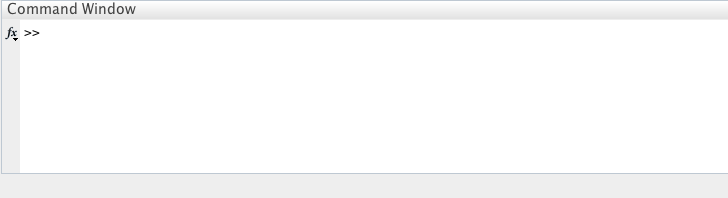
\includegraphics[scale=0.3]{images/pantalla2.png}
\end{center}
\begin{alertblock}{Importante}
La función clc no no limpia la ventana de command history.
\end{alertblock}
\end{frame}

\begin{frame}{Current directory}
Muestra todos los ficheros matlab en una carpeta de la computadora llamada directorio actual.
\begin{center}
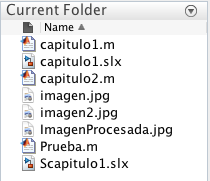
\includegraphics[scale=0.3]{images/pantalla4.png}
\end{center}
\end{frame}

\begin{frame}{Current directory}
Muestra todos los ficheros matlab en una carpeta de la computadora llamada directorio actual.
\begin{center}
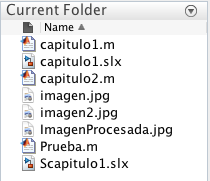
\includegraphics[scale=0.3]{images/pantalla4.png}
\end{center}
\begin{alertblock}{Importante}
Cuando MATLAB guarda información, usa el directorio actual a menos que se especifique algo diferente.
\end{alertblock}
\end{frame}

\begin{frame}{Workspace}
Mantiene informado las variables que se definen conforme se ejecuta comandos en la ventana de comandos, script o función.
\begin{center}
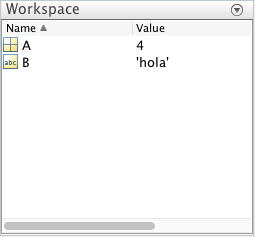
\includegraphics[scale=0.3]{images/pantalla5.png}
\end{center}
Ej. Ejecutar las siguiente líneas. Obtener conclusiones.
\lstinputlisting[xleftmargin=.4\textwidth]{scripts/ej2.m}
\begin{exampleblock}{Comando}
Ver comando: \textbf{clear}
\end{exampleblock}
\end{frame}

\begin{frame}{Help}
Muestra y busca documentación para la familia completa de productos MATLAB.
\begin{center}
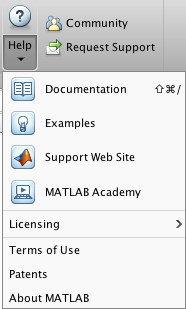
\includegraphics[scale=0.3]{images/pantalla6.png}
\end{center}
Buscar la ayuda de la función interna: sqrt \textit{(Square root)}
\end{frame}

\begin{frame}{Help}
\begin{center}
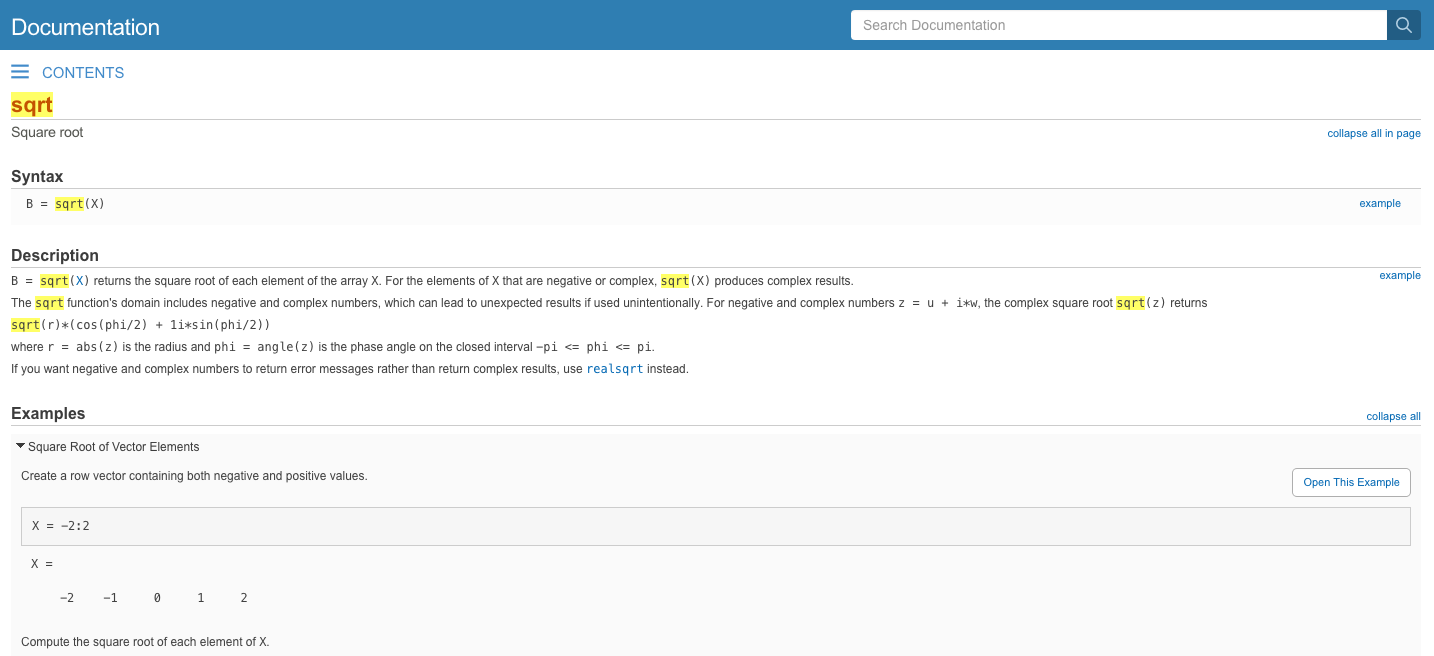
\includegraphics[scale=0.2]{images/pantalla7.png}
\end{center}
\end{frame}


\begin{frame}{Archivos .m}
\begin{center}
Existen dos tipos de archivos .m, llamados script y funciones
\end{center}
\end{frame}

\begin{frame}{Scripts}
\begin{itemize}
\item Un script es un programa. No posee argumentos de entrada ni salida
\item Operan con datos existentes en el directorio de trabajo o con nuevos datos creados por el script
\item Un programa es una secuencia de instrucciones ejecutables
\item Se guarda en un archivo .m en el directorio de trabajo
\item Se ejecuta abriendo el nombre del archivo en la consola o pulsando F5 en el editor. Otra forma es ejecutando el mismo en la ventana de edición
\end{itemize}
\end{frame}

\begin{frame}{Funciones}
\begin{center}

\includegraphics[scale=0.2]{images/stop.jpg}
\\\textit{Las estudiaremos más adelante}
\end{center}
\end{frame}

\end{document}
